\documentclass{beamer}
\usepackage[utf8]{inputenc}
\usepackage{graphicx, epsfig}
\usepackage{amsmath,mathrsfs,amsfonts,amssymb}
\usepackage{floatflt}
\usepackage{epic,ecltree}
\usepackage{mathtext}
\usepackage{fancybox}
\usepackage{fancyhdr}
\usepackage{multirow}
\usepackage{enumerate}
\usepackage{epstopdf}
\usepackage{multicol}
\usepackage{algorithm}
\usepackage[noend]{algorithmic}
\usepackage{tikz}
\usepackage{blindtext}
\usetheme{default}%{Singapore}%{Warsaw}%{Warsaw}%{Darmstadt}
\usecolortheme{default}

\setbeamerfont{title}{size=\Huge}
\setbeamertemplate{footline}[page number]{}

\setbeamertemplate{section in toc}[sections numbered]


\makeatletter
\newcommand\HUGE{\@setfontsize\Huge{35}{40}}
\makeatother    

\setbeamerfont{title}{size=\HUGE}
\beamertemplatenavigationsymbolsempty

% latin bold lower
\newcommand{\ba}{\mathbf{a}} 
\newcommand{\bc}{\mathbf{c}} 
\newcommand{\be}{\mathbf{e}} 
\newcommand{\bh}{\mathbf{h}} 
\newcommand{\bp}{\mathbf{p}} 
\newcommand{\bt}{\mathbf{t}} 
\newcommand{\bs}{\mathbf{s}} 
\newcommand{\bu}{\mathbf{u}} 
\newcommand{\bv}{\mathbf{v}} 
\newcommand{\bw}{\mathbf{w}} 
\newcommand{\bx}{\mathbf{x}} 
\newcommand{\by}{\mathbf{y}} 
\newcommand{\bz}{\mathbf{z}} 

% latin bold upper
\newcommand{\bA}{\mathbf{A}} 
\newcommand{\bB}{\mathbf{B}} 
\newcommand{\bC}{\mathbf{C}} 
\newcommand{\bI}{\mathbf{I}} 
\newcommand{\bJ}{\mathbf{J}} 
\newcommand{\bL}{\mathbf{L}} 
\newcommand{\bM}{\mathbf{M}} 
\newcommand{\bP}{\mathbf{P}}
\newcommand{\bQ}{\mathbf{Q}} 
\newcommand{\bR}{\mathbf{R}} 
\newcommand{\bT}{\mathbf{T}} 
\newcommand{\bU}{\mathbf{U}} 
\newcommand{\bV}{\mathbf{V}} 
\newcommand{\bW}{\mathbf{W}} 
\newcommand{\bX}{\mathbf{X}} 
\newcommand{\bY}{\mathbf{Y}} 
\newcommand{\bZ}{\mathbf{Z}} 

% latin cal upper
\newcommand{\cF}{\mathcal{F}} 
\newcommand{\cG}{\mathcal{G}} 
\newcommand{\cI}{\mathcal{I}} 
\newcommand{\cL}{\mathcal{L}} 
\newcommand{\cM}{\mathcal{M}} 
\newcommand{\cN}{\mathcal{N}} 
\newcommand{\cS}{\mathcal{S}} 
\newcommand{\cT}{\mathcal{T}} 
\newcommand{\cW}{\mathcal{W}} 
\newcommand{\cX}{\mathcal{X}} 
\newcommand{\cZ}{\mathcal{Z}} 

% latin bb upper
\newcommand{\bbE}{\mathbb{E}} 
\newcommand{\bbI}{\mathbb{I}} 
\newcommand{\bbP}{\mathbb{P}} 
\newcommand{\bbR}{\mathbb{R}} 

% greek bold lower
\newcommand{\bepsilon}{\boldsymbol{\epsilon}} 
\newcommand{\btheta}{\boldsymbol{\theta}} 
\newcommand{\blambda}{\boldsymbol{\lambda}} 
\newcommand{\bpi}{\boldsymbol{\pi}} 
\newcommand{\bmu}{\boldsymbol{\mu}} 
\newcommand{\bsigma}{\boldsymbol{\sigma}} 
\newcommand{\bphi}{\boldsymbol{\phi}} 

% greek bold upper
\newcommand{\bSigma}{\boldsymbol{\Sigma}} 

\DeclareMathOperator*{\argmin}{arg\,min}
\DeclareMathOperator*{\argmax}{arg\,max}

\newcommand{\createdgmtitle}[1]{\title[\hbox to 56mm{Deep Generative Models  \hfill\insertframenumber\,/\,\inserttotalframenumber}]
	{\vspace{1cm} \\ Deep Generative Models \\ {\Huge Lecture #1}}
	\author{Roman Isachenko}
	\institute{
	Moscow Institute of Physics and Technology
	} 
	\date{2023, Autumn}
}

\usepackage{tikz}
\usetikzlibrary{arrows,shapes,positioning,shadows,trees}

\newcommand\myfootnote[1]{%
  \tikz[remember picture,overlay]
  \draw (current page.south west) +(1in + \oddsidemargin,0.5em)
  node[anchor=south west,inner sep=0pt]{\parbox{\textwidth}{%
      \rlap{\rule{10em}{0.4pt}}\raggedright\scriptsize \textit{#1}}};}

\newcommand\myfootnotewithlink[2]{%
  \tikz[remember picture,overlay]
  \draw (current page.south west) +(1in + \oddsidemargin,0.5em)
  node[anchor=south west,inner sep=0pt]{\parbox{\textwidth}{%
      \rlap{\rule{10em}{0.4pt}}\raggedright\scriptsize\href{#1}{\textit{#2}}}};}
      
\AtBeginSection[]
      {
      	\begin{frame}{Outline}
      		\tableofcontents[currentsection]
      	\end{frame}
      }
      \AtBeginSubsection[]{
      	\begin{frame}{Outline}
      		\tableofcontents[currentsection,currentsubsection]
      	\end{frame}
}
\createdgmtitle{2}

\usepackage{tikz}

\usetikzlibrary{arrows,shapes,positioning,shadows,trees}
%--------------------------------------------------------------------------------
\begin{document}
%--------------------------------------------------------------------------------
\begin{frame}[noframenumbering,plain]
	%\thispagestyle{empty}
	\titlepage
\end{frame}
%=======
\begin{frame}{Recap of previous lecture}
	We are given i.i.d. samples $\{\bx_i\}_{i=1}^n \in \cX$ (e.g. $\cX = \bbR^m$) from unknown distribution $\pi(\bx)$.

	\begin{block}{Goal}
		We would like to learn a distribution $\pi(\bx)$ for 
		\begin{itemize}
		    \item evaluating $\pi(\bx)$ for new samples (how likely to get object $\bx$?);
		    \item sampling from $\pi(\bx)$ (to get new objects $\bx \sim \pi(\bx)$).
		\end{itemize}
	\end{block}
	Instead of searching true $\pi(\bx)$ over all probability distributions, learn function approximation $p(\bx | \btheta) \approx \pi(\bx)$.
	\begin{block}{Divergence}
		\begin{itemize}
			\item $D(\pi || p) \geq 0$ for all $\pi, p \in \cS$;
			\item $D(\pi || p) = 0$ if and only if $\pi \equiv p$.
		\end{itemize}
	\end{block}
	\begin{block}{Divergence minimization task}
		\vspace{-0.3cm}
		\[
		\min_{\btheta} D(\pi || p).
		\]
	\end{block}
\end{frame}
%=======
\begin{frame}{Recap of previous lecture}
	\begin{block}{Forward KL}
		\vspace{-0.2cm}
		\[
		KL(\pi || p) = \int \pi (\bx) \log \frac{\pi(\bx)}{p(\bx | \btheta)} d \bx \rightarrow \min_{\btheta}
		\]
	\end{block}
	\begin{block}{Reverse KL}
		\vspace{-0.2cm}
		\[
		KL(p || \pi) = \int p (\bx| \btheta) \log \frac{p(\bx| \btheta)}{\pi(\bx)} d \bx \rightarrow \min_{\btheta}
		\]
	\end{block}
	
	\begin{block}{Maximum likelihood estimation (MLE)}
		\vspace{-0.5cm}
		\[
		\btheta^* = \argmax_{\btheta} p(\bX | \btheta) = \argmax_{\btheta} \prod_{i=1}^n p(\bx_i | \btheta) = \argmax_{\btheta} \sum_{i=1}^n \log p(\bx_i | \btheta).
		\]
		\vspace{-0.1cm}
	\end{block}
	Maximum likelihood estimation is equivalent to minimization of the Monte-Carlo estimate of forward KL.
\end{frame}
%=======
\begin{frame}{Recap of previous lecture}
	\begin{block}{Likelihood as product of conditionals}
		Let $\bx = (x_1, \dots, x_m)$, $\bx_{1:j} = (x_1, \dots, x_j)$. Then 
		\[
		p(\bx | \btheta) = \prod_{j=1}^m p(x_j | \bx_{1:j - 1}, \btheta); \quad 
		\log p(\bx | \btheta) = \sum_{j=1}^m \log p(x_j | \bx_{1:j - 1}, \btheta).
		\]
	\end{block}
	\vspace{-0.3cm}
	\begin{block}{MLE problem for autoregressive model}
		\vspace{-0.5cm}
		\[
		\btheta^* = \argmax_{\btheta} p(\bX | \btheta) = \argmax_{\btheta} \sum_{i=1}^n \sum_{j=1}^m \log p(x_{ij} | \bx_{i, 1:j - 1}\btheta).
		\]
		\vspace{-0.5cm}
	\end{block}
	\begin{block}{Sampling}
		\vspace{-0.5cm}
		\[
		{\color{teal}\hat{x}_1} \sim p(x_1 | \btheta), \quad \hat{x}_2 \sim p(x_2 | {\color{teal}\hat{x}_1}, \btheta), \quad \dots, \quad \hat{x}_m \sim p(x_m | \hat{\bx}_{1:m-1}, \btheta)
		\]
		New generated object is $\hat{\bx} = (\hat{x}_1, \hat{x}_2, \dots, \hat{x}_m)$.
	\end{block}
\end{frame}
%=======
\begin{frame}{Recap of previous lecture}
	\begin{block}{Autoregressive MLP}
		\vspace{-0.3cm}
 		\begin{figure}
		     \centering
		     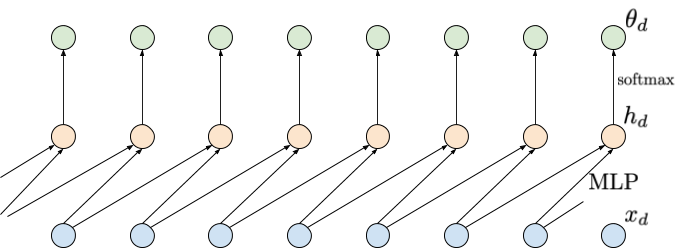
\includegraphics[width=0.6\linewidth]{figs/sequential_MLP}
		 \end{figure}
	\end{block}
	\vspace{-0.3cm}

	\begin{block}{Autoregressive CNN}
		\begin{minipage}[t]{0.5\columnwidth}
			\begin{figure}
				\centering
	      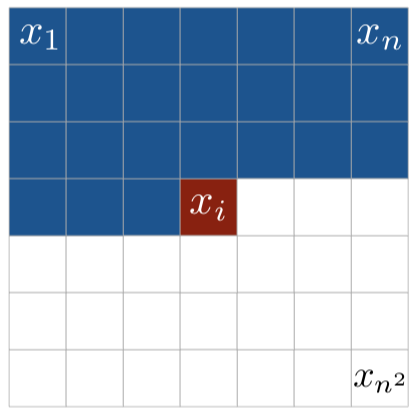
\includegraphics[width=0.6\linewidth]{figs/pixelcnn1}
			\end{figure}
		\end{minipage}%
		\begin{minipage}[t]{0.5\columnwidth}
			\begin{figure}
				\centering
	      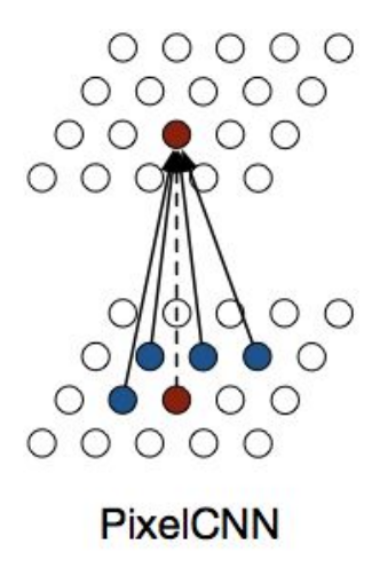
\includegraphics[width=0.45\linewidth]{figs/pixelcnn_0_2}
			\end{figure}
		\end{minipage}
	\end{block}
	 \myfootnotewithlink{https://jmtomczak.github.io/blog/2/2\_ARM.html}{image credit: https://jmtomczak.github.io/blog/2/2\_ARM.html}
\end{frame}
%=======
\begin{frame}{Outline}
    \tableofcontents
\end{frame}
%=======
\begin{frame}{Generative models zoo}
	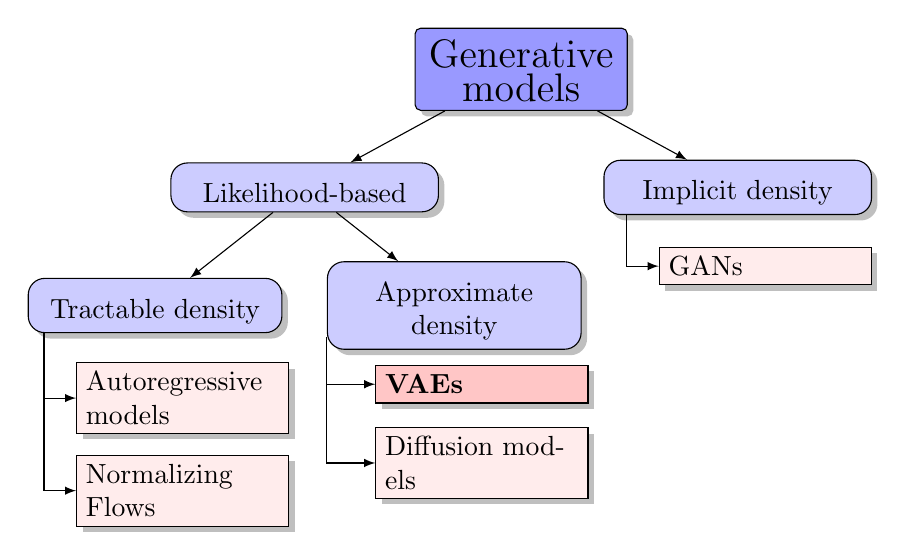
\begin{tikzpicture}[
	 	basic/.style  = {draw, text width=2cm, drop shadow, rectangle},
	 	root/.style   = {basic, rounded corners=2pt, thin, text height=1.1em, text width=7em, align=center, fill=blue!40},
	 	level 1/.style={sibling distance=55mm},
	 	level 2/.style = {basic, rounded corners=6pt, thin, align=center, fill=blue!20, text height=1.1em, text width=9em, sibling distance=38mm},
	 	level 3/.style = {basic, rounded corners=6pt, thin,align=center, fill=blue!20, text width=8.5em},
	 	level 4/.style = {basic, thin, align=left, fill=pink!30, text width=7em},
	 	level 5/.style = {basic, thin, align=left, fill=pink!90, text width=7em},
		edge from parent/.style={->,draw},
		>=latex]
		
		% root of the the initial tree, level 1
		\node[root] {\Large Generative models}
		% The first level, as children of the initial tree
		child {node[level 2] (c1) {Likelihood-based}
			child {node[level 3] (c11) {Tractable density}}
			child {node[level 3] (c12) {Approximate density}}
		}
		child {node[level 2] (c2) {Implicit density}};
		
		% The second level, relatively positioned nodes
		\begin{scope}[every node/.style={level 5}]
		\node [below of = c12, xshift=10pt] (c121) {\textbf{VAEs}};
		\end{scope}
	
		% The second level, relatively positioned nodes
		\begin{scope}[every node/.style={level 4}]
			\node [below of = c11, yshift=-5pt, xshift=10pt] (c111) {Autoregressive models};
			\node [below of = c111, yshift=-5pt] (c112) {Normalizing Flows};
			
			\node [below of = c121] (c122) {Diffusion models};
			
			\node [below of = c2, xshift=10pt] (c21) {GANs};
		\end{scope}
	
		
		% lines from each level 1 node to every one of its "children"
		\foreach \value in {1,2}
		\draw[->] (c11.194) |- (c11\value.west);
		
		\foreach \value in {1,2}
		\draw[->] (c12.194) |- (c12\value.west);
		
		\draw[->] (c2.194) |- (c21.west);
		
	\end{tikzpicture}
\end{frame}
%=======
\section{Bayesian framework}
%=======
\begin{frame}{Bayesian framework}
	\begin{block}{Bayes theorem}
		\[
			p(\bt | \bx) = \frac{p(\bx | \bt) p(\bt)}{p(\bx)} = \frac{p(\bx | \bt) p(\bt)}{\int p(\bx | \bt) p(\bt) d \bt} 
		\]
		\begin{itemize}
			\item $\bx$ -- observed variables, $\bt$ -- unobserved variables (latent variables/parameters);
			\item $p(\bx | \bt)$ -- likelihood;
			\item $p(\bx) = \int p(\bx | \bt) p(\bt) d \bt$ -- evidence;
			\item $p(\bt)$ -- prior distribution, $p(\bt | \bx)$ -- posterior distribution.
		\end{itemize}
	\end{block}
	\begin{block}{Meaning}
		We have unobserved variables $\bt$ and some prior knowledge about them $p(\bt)$. Then, the data $\bx$ has been observed. 
		Posterior distribution $p(\bt | \bx)$ summarizes the knowledge after the observations.
	\end{block}
\end{frame}
%=======
\begin{frame}{Bayesian framework}
	Let consider the case, where the unobserved variables $\bt$ is our model parameters $\btheta$.
	\begin{itemize}
		\item $\bX = \{\bx_i\}_{i=1}^n$ -- observed samples;
		\item $p(\btheta)$ -- prior parameters distribution (we treat model parameters $\btheta$ as random variables).
	\end{itemize}
	\begin{block}{Posterior distribution}
		\[
			p(\btheta | \bX) = \frac{p(\bX | \btheta) p(\btheta)}{p(\bX)} = \frac{p(\bX | \btheta) p(\btheta)}{\int p(\bX | \btheta) p(\btheta) d \btheta} 
		\]
		\vspace{-0.2cm}
	\end{block}
	\begin{block}{Bayesian inference}
		\vspace{-0.2cm}
		\[
			p(\bx | \bX) = \int p(\bx | \btheta) p(\btheta | \bX) d \btheta
		\]
	\end{block}
 	Note the difference from
	 	\[
	 		p(\bx) = \int p(\bx | \btheta) p(\btheta) d \btheta.
	 	\]
\end{frame}
%=======
\begin{frame}{Bayesian framework}
	\begin{block}{Posterior distribution}
		\[
		p(\btheta | \bX) = \frac{p(\bX | \btheta) p(\btheta)}{p(\bX)} = \frac{p(\bX | \btheta) p(\btheta)}{\int p(\bX | \btheta) p(\btheta) d \btheta} 
		\]
		\vspace{-0.2cm}
	\end{block}
	\begin{block}{Bayesian inference}
		\vspace{-0.2cm}
		\[
		p(\bx | \bX) = \int p(\bx | \btheta) p(\btheta | \bX) d \btheta
		\]
	\end{block}
	If evidence $p(\bX)$ is intractable (due to multidimensional integration), we can't get posterior distribution and perform the precise inference.
    \begin{block}{Maximum a posteriori (MAP) estimation}
    \vspace{-0.2cm}
    \[
        \btheta^* = \argmax_{\btheta} p(\btheta | \bX) = \argmax_{\btheta} \bigl(\log p(\bX | \btheta) + \log p(\btheta) \bigr)
    \]
    \end{block}
\end{frame}
%=======
\begin{frame}{Bayesian framework}
	\begin{block}{MAP estimation}
		\vspace{-0.2cm}
		\[
		\btheta^* = \argmax_{\btheta} p(\btheta | \bX) = \argmax_{\btheta} \bigl(\log p(\bX | \btheta) + \log p(\btheta) \bigr)
		\]
	\end{block}
	Estimated $\btheta^*$ is a deterministic variable, but we could treat it as a random variable with density $p(\btheta | \bX) = \delta(\btheta - \btheta^*)$.
	\begin{block}{Dirac delta function}
		\[
			\delta(x) = 
			\begin{cases}
				+\infty, \quad x = 0; \\
				0, \quad x \neq 0;
			\end{cases} \, 
			\int \delta(x) dx = 1; \,\, 
			\int f(x) \delta (x - y) dx = f(y).
		\]
	\end{block}
	\begin{block}{MAP inference}
		\[
			p(\bx | \bX) = \int p(\bx| \btheta) p(\btheta | \bX ) d \btheta \approx p(\bx | \btheta^*).
		\]
	\end{block}
\end{frame}
%=======
\section{Latent variable models (LVM)}
%=======
\begin{frame}{Latent variable models (LVM)}
	\begin{block}{MLE problem}
		\vspace{-0.5cm}
		\[
		\btheta^* = \argmax_{\btheta} p(\bX | \btheta) = \argmax_{\btheta} \prod_{i=1}^n p(\bx_i | \btheta) = \argmax_{\btheta} \sum_{i=1}^n \log p(\bx_i | \btheta).
		\]
		\vspace{-0.5cm}
	\end{block}
	The distribution $p(\bx | \btheta)$ could be very complex and intractable (as well as real distribution $\pi(\bx)$).
	\begin{block}{Extended probabilistic model}
		Introduce latent variable $\bz$ for each sample $\bx$
		\[
		p(\bx, \bz | \btheta) = p(\bx | \bz, \btheta) p(\bz); \quad 
		\log p(\bx, \bz | \btheta) = \log p(\bx | \bz, \btheta) + \log p(\bz).
		\]
		\[
		p(\bx | \btheta) = \int p(\bx, \bz | \btheta) d\bz = \int p(\bx | \bz, \btheta) p(\bz) d\bz.
		\]
	\end{block}
	\vspace{-0.3cm}
	\begin{block}{Motivation}
		The distributions $p(\bx | \bz, \btheta)$ and $p(\bz)$ could be quite simple.
	\end{block}
\end{frame}
%=======
\begin{frame}{Latent variable models (LVM)}
	\[
	\log p(\bx | \btheta) = \log \int p(\bx | \bz, \btheta) p(\bz) d\bz \rightarrow \max_{\btheta}
	\]
	\vspace{-0.6cm}
	\begin{block}{Examples}
		\begin{minipage}[t]{0.45\columnwidth}
			\textit{Mixture of gaussians} \\
			\vspace{-0.5cm}
			\begin{figure}
				\centering
				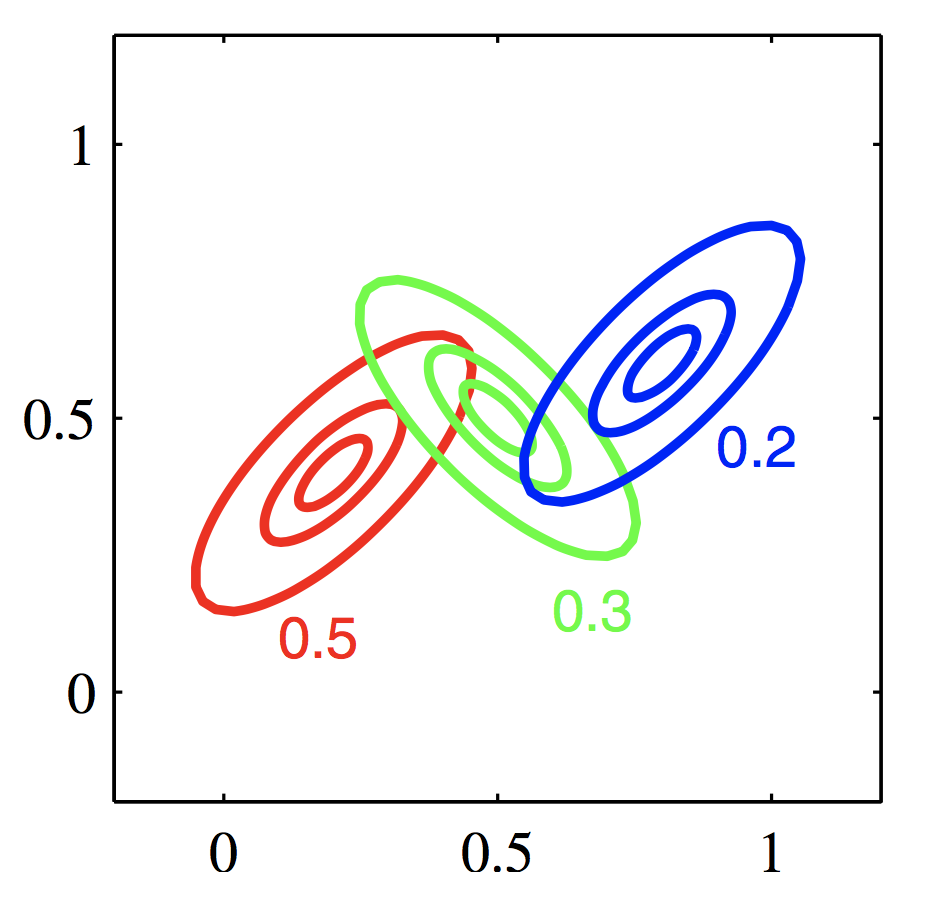
\includegraphics[width=0.75\linewidth]{figs/mixture_of_gaussians}
			\end{figure}
			\vspace{-0.5cm}
			\begin{itemize}
				\item $p(\bx | z, \btheta) = \cN(\bx | \bmu_z, \bSigma_z)$
				\item $p(z) = \text{Categorical}(\bpi)$
			\end{itemize}
		\end{minipage}%
		\begin{minipage}[t]{0.53\columnwidth}
			\textit{PCA model} \\
			\vspace{-0.5cm}
			\begin{figure}
				\centering
				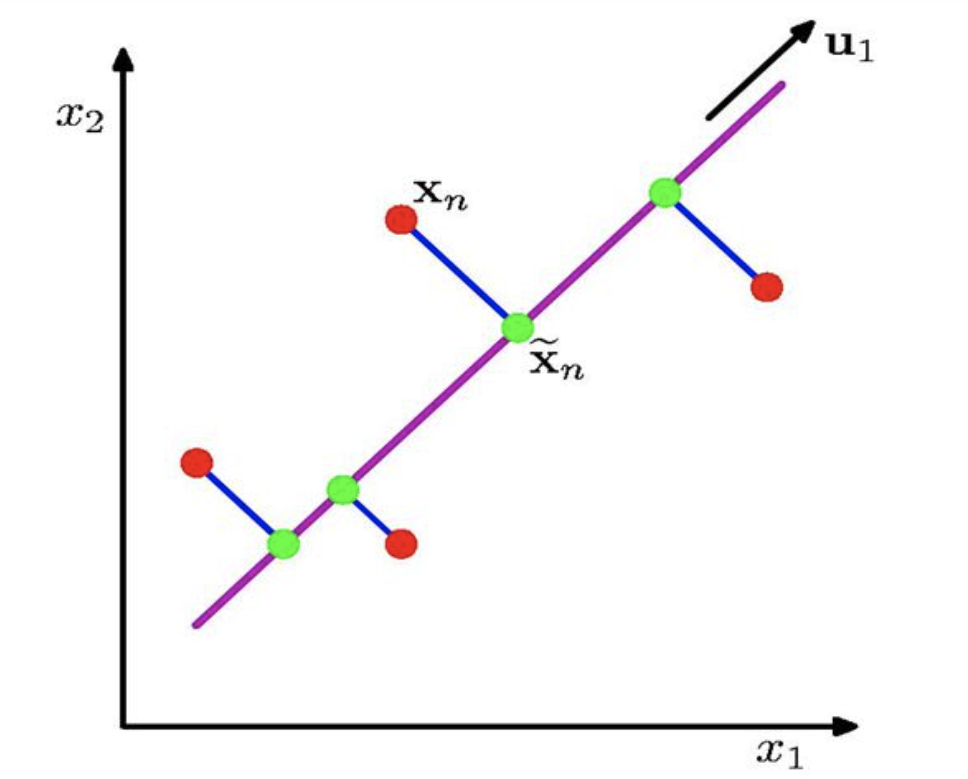
\includegraphics[width=.7\linewidth]{figs/pca}
			\end{figure}
			\vspace{-0.3cm}
			\begin{itemize}
				\item $p(\bx | \bz, \btheta) = \cN(\bx | \bW \bz + \bmu, \sigma^2 \bI)$
				\item $p(\bz) = \cN(\bz | 0, \bI)$
			\end{itemize}
		\end{minipage}
	\end{block}
	\myfootnote{Bishop\,C. Pattern Recognition and Machine Learning, 2006}
\end{frame}
%=======
\begin{frame}{Latent variable models (LVM)}
	\[
	\log p(\bx | \btheta) = \log \int p(\bx | \bz, \btheta) p(\bz) d\bz \rightarrow \max_{\btheta}
	\]
	\textbf{PCA} projects original data $\bX$ onto a low dimensional latent space while maximizing the variance of the projected data. 
	\begin{figure}
		\centering
		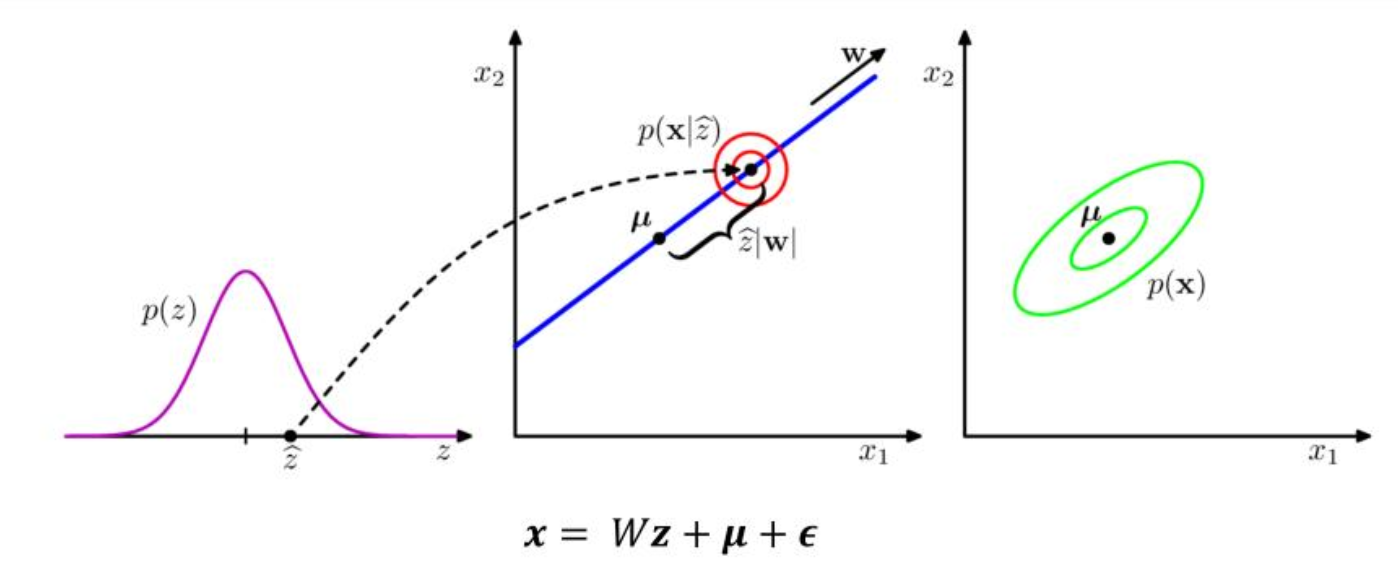
\includegraphics[width=.7\linewidth]{figs/bayesian_pca}
	\end{figure}
	\vspace{-0.5cm}
	\begin{itemize}
		\item $p(\bx | \bz, \btheta) = \cN(\bx | \bW \bz + \bmu, \sigma^2 \bI)$
		\item $p(\bz) = \cN(\bz | 0, \bI)$
		\item $p(\bx) = \cN(\bx | \bmu, \bW \bW^T + \sigma^2 \bI)$
		\item $p(\bz | \bx) = \cN \bigl(\bM^{-1} \bW^T (\bx - \bmu), \sigma^2 \bM\bigr)$, where $\bM = \bW \bW^T + \sigma^2 \bI$
	\end{itemize}
\end{frame}
%=======
\begin{frame}{Maximum likelihood estimation for LVM}
	\begin{block}{MLE for extended problem}
		\vspace{-0.7cm}
		\begin{multline*}
			\vspace{-0.5cm}
			\btheta^* = \argmax_{\btheta} p(\bX, \bZ | \btheta) = \argmax_{\btheta} \prod_{i=1}^n p(\bx_i, \bz_i | \btheta) = \\ = \argmax_{\btheta} \sum_{i=1}^n \log p(\bx_i, \bz_i | \btheta).
		\end{multline*}
		\vspace{-0.5cm}
	\end{block}
	However, $\bZ$ is unknown.
	\begin{block}{MLE for original problem}
		\vspace{-0.7cm}
		\begin{multline*}
			\btheta^* = \argmax_{\btheta} \log p(\bX| \btheta) = \argmax_{\btheta} \sum_{i=1}^n \log p(\bx_i | \btheta) = \\ =  \argmax_{\btheta}  \sum_{i=1}^n \log \int p(\bx_i, \bz_i | \btheta) d \bz_i = \\ = \argmax_{\btheta} \log \sum_{i=1}^n \int p(\bx_i| \bz_i, \btheta) p(\bz_i) d\bz_i.
		\end{multline*}
	\end{block}
	
\end{frame}
%=======
\begin{frame}{Naive approach}
	\begin{figure}
		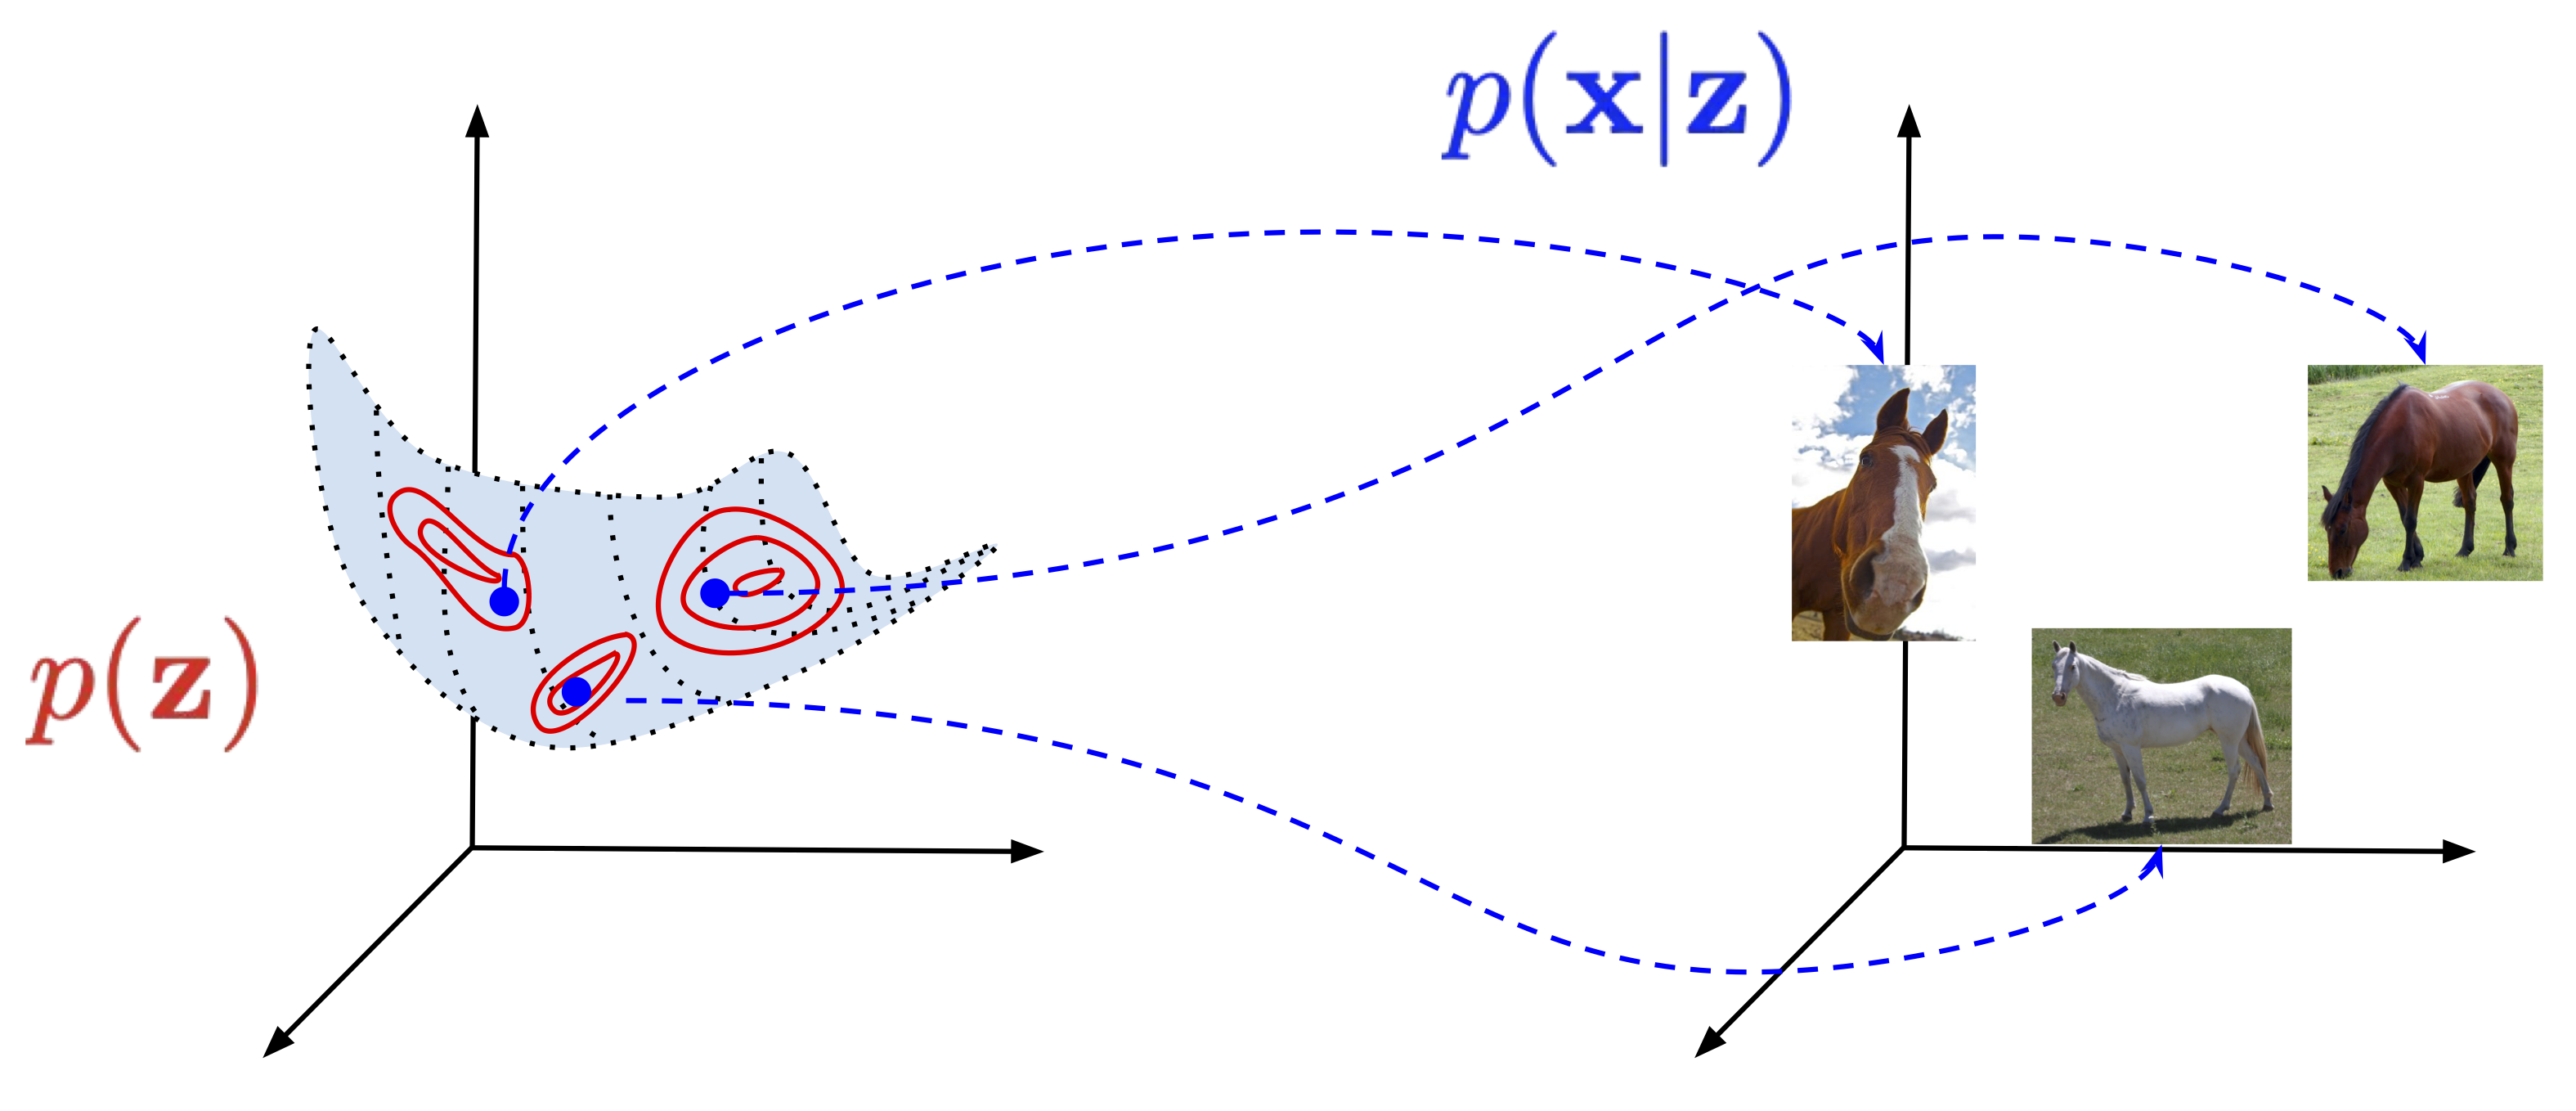
\includegraphics[width=.75\linewidth]{figs/lvm_diagram}
	\end{figure}
	\begin{block}{Monte-Carlo estimation}
		\vspace{-0.7cm}
		\[
			p(\bx | \btheta) = \int p(\bx | \bz, \btheta) p(\bz) d\bz = \bbE_{p(\bz)} p(\bx | \bz, \btheta) \approx \frac{1}{K} \sum_{k=1}^{K} p(\bx | \bz_k, \btheta),
		\]
		\vspace{-0.5cm} \\
		where $\bz_k \sim p(\bz)$. \\
		\textbf{Challenge:} to cover the space properly, the number of samples grows exponentially with respect to dimensionality of $\bz$. 
	\end{block}
	\myfootnotewithlink{https://jmtomczak.github.io/blog/4/4\_VAE.html}{image credit: https://jmtomczak.github.io/blog/4/4\_VAE.html}
\end{frame}
%=======
\section{Variational lower bound (ELBO)}
%=======
\begin{frame}{Variational lower bound (ELBO)}
	\begin{block}{Derivation 1 (inequality)}
		\vspace{-0.7cm}
		\begin{multline*}
			\log p(\bx| \btheta) 
			= \log \int p(\bx, \bz | \btheta) d\bz = \log \int \frac{q(\bz)}{q(\bz)} p(\bx, \bz | \btheta) d\bz = \\
			= \log \bbE_{q} \left[\frac{p(\bx, \bz| \btheta)}{q(\bz)} \right] \geq \bbE_{q} \log \frac{p(\bx, \bz| \btheta)}{q(\bz)} =  \cL(q, \btheta)
		\end{multline*}
		\vspace{-0.7cm}
	\end{block}
	\begin{block}{Derivation 2 (equality)}
		\vspace{-0.7cm}
		\begin{multline*}
			\mathcal{L} (q, \btheta) = \int q(\bz) \log \frac{p(\bx, \bz | \btheta)}{q(\bz)}d\bz = 
			\int q(\bz) \log \frac{p(\bz|\bx, \btheta)p(\bx| \btheta)}{q(\bz)}d\bz = \\
			= \int q(\bz) \log p(\bx| \btheta) d\bz + \int q(\bz) \log \frac{p(\bz|\bx, \btheta)}{q(\bz)}d\bz = \\
			= \log p(\bx| \btheta) - KL(q(\bz) || p(\bz|\bx, \btheta))
		\end{multline*}
	\end{block}
	\vspace{-0.7cm}
	\begin{block}{Variational decomposition}
		\[
			\log p(\bx| \btheta) = \mathcal{L} (q, \btheta) + KL(q(\bz) || p(\bz|\bx, \btheta)) \geq \mathcal{L} (q, \btheta).
		\]
	\end{block}
\end{frame}
%=======
\begin{frame}{Variational lower bound (ELBO)}
	\vspace{-0.3cm}
	\begin{align*}
		\mathcal{L} (q, \btheta) &= \int q(\bz) \log \frac{\color{violet}p(\bx, \bz | \btheta)}{\color{teal}q(\bz)}d\bz = \\ 
		&= \int q(\bz) \log {\color{violet}p(\bx | \bz, \btheta)} d\bz + \int q(\bz) \log \frac{\color{violet}p(\bz)}{\color{teal}q(\bz)}d\bz \\ 
		&= \mathbb{E}_{q} \log p(\bx | \bz, \btheta) - KL (q(\bz) || p(\bz))
	\end{align*}
	\vspace{-0.5cm}
	\begin{block}{Log-likelihood decomposition}
		\vspace{-0.8cm}
		\begin{multline*}
			\log p(\bx| \btheta) = {\color{olive}\mathcal{L} (q, \btheta)} + KL(q(\bz) || p(\bz|\bx, \btheta)) \\ = {\color{olive}\mathbb{E}_{q} \log p(\bx | \bz, \btheta) - KL (q(\bz) || p(\bz))} + KL(q(\bz) || p(\bz|\bx, \btheta)).
		\end{multline*}
		\vspace{-0.7cm}
	\end{block}
	\begin{itemize}
		\item Instead of maximizing incomplete likelihood, maximize ELBO
		\[
		\max_{\btheta} p(\bx | \btheta) \quad \rightarrow \quad \max_{q, \btheta} \mathcal{L} (q, \btheta)
		\]
		\item Maximization of ELBO by \textbf{variational} distribution $q$ is equivalent to minimization of KL
		\[
		\argmax_q \mathcal{L} (q, \btheta) \equiv \argmin_q KL(q(\bz) || p(\bz|\bx, \btheta)).
		\]
	\end{itemize}
\end{frame}
%=======
\section{EM-algorithm, amortized inference}
%=======
\begin{frame}{EM-algorithm}
	\vspace{-0.5cm}
	\begin{multline*}
		\mathcal{L} (q, \btheta)  =  \mathbb{E}_{q} \log p(\bx | \bz, \btheta) - KL (q(\bz) || p(\bz)) = \\ = \bbE_q \left[ \log p(\bx | \bz, \btheta) - \log \frac{q(\bz)}{p(\bz)} \right]d\bz \rightarrow \max_{q, \btheta}.
	\end{multline*}
	\vspace{-0.5cm}
	\begin{block}{Block-coordinate optimization}
		\begin{itemize}
			\item Initialize $\btheta^*$;
			\item \textbf{E-step} ($\mathcal{L} (q, \btheta) \rightarrow \max_q$)
			\vspace{-0.2cm}
			\begin{multline*}
				q^*(\bz) = \argmax_q \mathcal{L} (q, \btheta^*) = \\
				= \argmin_q KL(q(\bz) || p(\bz | \bx, \btheta^*)) = p(\bz| \bx, \btheta^*);
			\end{multline*}
			\item \textbf{M-step} ($\mathcal{L} (q, \btheta) \rightarrow \max_{\btheta}$)
			\vspace{-0.2cm}
			\[
			\btheta^* = \argmax_{\btheta} \mathcal{L} (q^*, \btheta);
			\]
			\vspace{-0.2cm}
			\item Repeat E-step and M-step until convergence.
		\end{itemize}
	\end{block}
\end{frame}
%=======
\begin{frame}{EM-algorithm illustration}
	
	\begin{minipage}[t]{0.45\columnwidth}
		\begin{figure}
			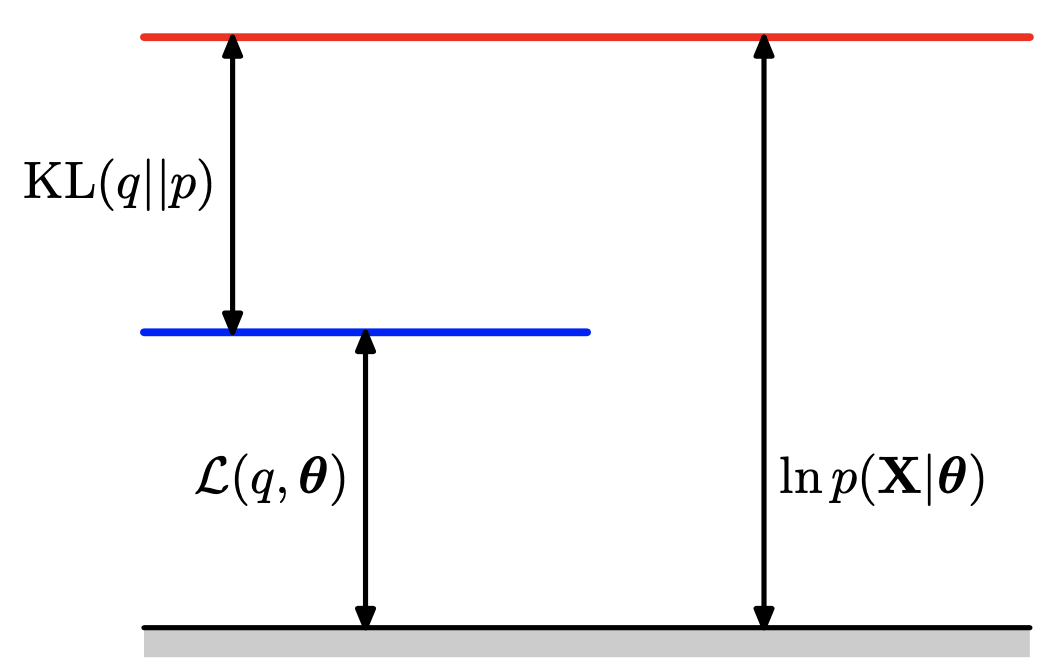
\includegraphics[width=0.9\linewidth]{figs/em_bishop1}
		\end{figure}
	\end{minipage}%
	\begin{minipage}[t]{0.55\columnwidth}
		\begin{figure}
			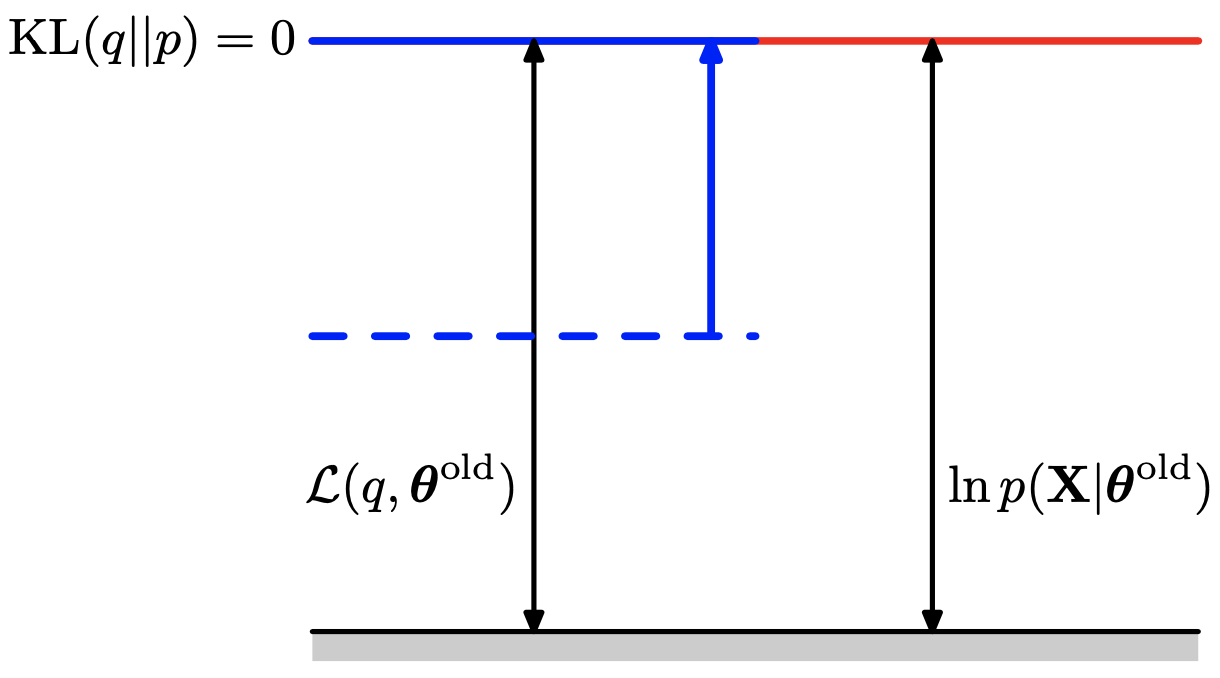
\includegraphics[width=0.85\linewidth]{figs/em_bishop2}
		\end{figure}
	\end{minipage}
	\begin{figure}
		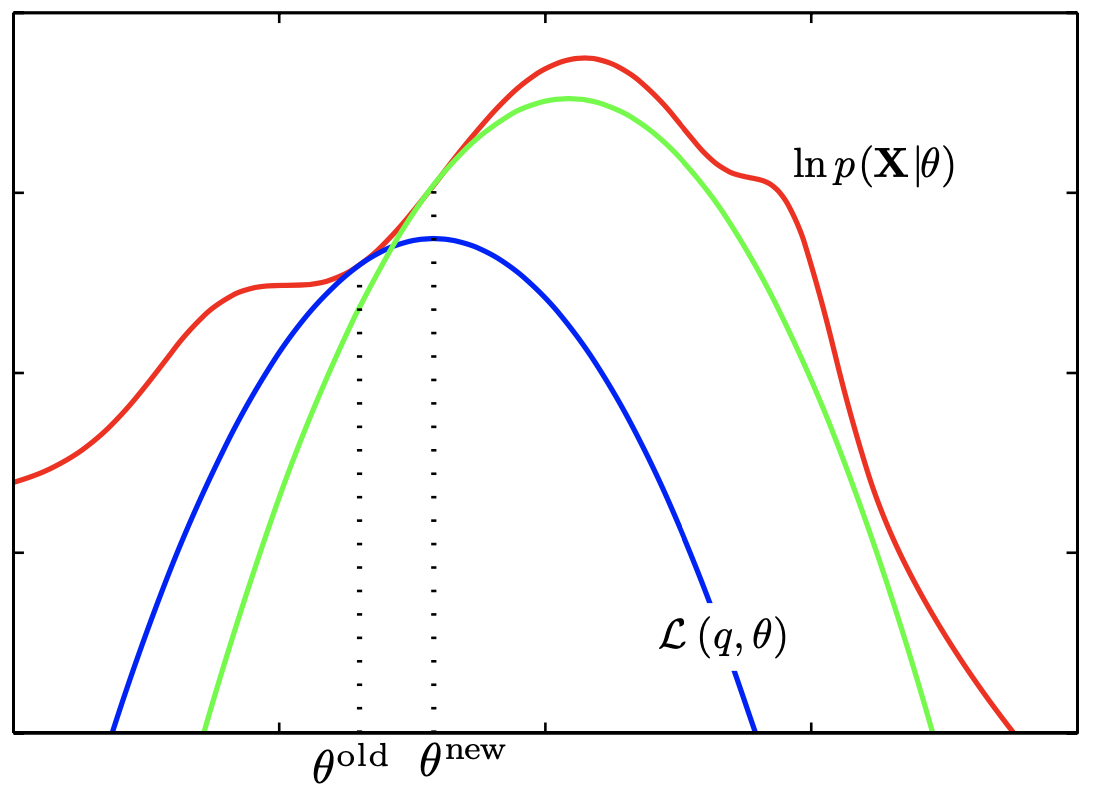
\includegraphics[width=.55\linewidth]{figs/em_bishop3}
	\end{figure}
	
	\myfootnote{Bishop\,C. Pattern Recognition and Machine Learning, 2006}
\end{frame}
%=======
\begin{frame}{Amortized variational inference}
	\begin{block}{E-step}
		\vspace{-0.3cm}
		\[
		q(\bz) = \argmax_q \mathcal{L} (q, \btheta^*) = \argmin_q KL(q || p) =
		p(\bz| \bx, \btheta^*).
		\]
		\vspace{-0.3cm}
		\begin{itemize}
			\item $q(\bz)$ approximates true posterior distribution $p(\bz| \bx, \btheta^*)$, that is why it is called \textbf{variational posterior};
			\item $p(\bz| \bx, \btheta^*)$ could be \textbf{intractable};
			\item $q(\bz)$ is different for each object $\bx$.
		\end{itemize}
		\vspace{-0.3cm}
	\end{block}
	\begin{block}{Idea}
		Restrict a family of all possible distributions $q(\bz)$ to a parametric class $q(\bz|\bx, \bphi)$ conditioned on samples $\bx$ with parameters $\bphi$.
	\end{block}
	
	\textbf{Variational Bayes}
	\begin{itemize}
		\item E-step
		\[
		\bphi_k = \bphi_{k-1} + \left.\eta \nabla_{\bphi} \mathcal{L}(\bphi, \btheta_{k-1})\right|_{\bphi=\bphi_{k-1}}
		\]
		\item M-step
		\[
		\btheta_k = \btheta_{k-1} + \left.\eta \nabla_{\btheta} \mathcal{L}(\bphi_k, \btheta)\right|_{\btheta=\btheta_{k-1}}
		\]
	\end{itemize}
\end{frame}
%=======
\begin{frame}{Variational EM-algorithm}
	\begin{block}{ELBO}
		\vspace{-0.5cm}
		\[
		\log p(\bx| \btheta) = \mathcal{L} (\bphi, \btheta) + KL(q(\bz | \bx, \bphi) || p(\bz|\bx, \btheta)) \geq \mathcal{L} (\bphi, \btheta).
		\]
		\vspace{-0.5cm}
	\end{block}
	\begin{itemize}
		\item \textbf{E-step}
		\[
		\bphi_k = \bphi_{k-1} + \left.\eta \nabla_{\bphi} \mathcal{L}(\bphi, \btheta_{k-1})\right|_{\bphi=\bphi_{k-1}},
		\]
		where $\bphi$~-- parameters of variational posterior distribution $q(\bz | \bx, \bphi)$.
		\item \textbf{M-step}
		\[
		\btheta_k = \btheta_{k-1} + \left.\eta \nabla_{\btheta} \mathcal{L}(\bphi_k, \btheta)\right|_{\btheta=\btheta_{k-1}},
		\]
		where $\btheta$~-- parameters of the generative distribution $p(\bx | \bz, \btheta)$.
	\end{itemize}
	Now all we have to do is to obtain two gradients $\nabla_{\bphi} \mathcal{L}(\bphi, \btheta)$, $\nabla_{\btheta} \mathcal{L}(\bphi, \btheta)$.  \\
	\textbf{Challenge:} Number of samples $n$ could be huge (we heed to derive unbiased stochastic gradients).
\end{frame}
%=======
\begin{frame}{Summary}
	\begin{itemize}
		\item Bayesian inference is a generalization of most common machine learning tasks. It allows to construct MLE, MAP and bayesian inference, to compare models complexity and many-many more cool stuff.
		\vfill
		\item LVM introduces latent representation of observed samples to make model more interpretable.
		\vfill
		\item LVM maximizes variational evidence lower bound (ELBO) to find MLE for the parameters.
		\vfill
		\item The general variational EM algorithm maximizes ELBO objective for LVM model to find MLE for parameters $\btheta$.
	\end{itemize}
\end{frame}
\end{document} 